\section{Construction Grammar}
{\tiny like LFG and HPSG, Construction Grammar forms part of West Coast linguistics. It has been considerably influenced by Charles Fillmore, Paul Key and George Lakoff and Adele Goldberg}\\
\scriptsize{Goldbergian Construction Grammar}\\
\scriptsize{Construction} {\tiny Any linguistic pattern is recognized as a construction as long as some aspect of its form or function is not strictly predictable from its component parts or from other constructions recognized to exist\\
patterns are stored as constructions even if they are fully predictable as long as they occur with sufficient frequency, e.g. What be[fin] X doing Y?\\
all levels of grammatical analysis involve constructions: morpheme, word, complex word, idiom, covariational conditional, ditransitive, passive
}\\
\scriptsize{Notational Confusion} {\tiny for consistency, we use POS symbols, if necessary, can be further specified by indices\\
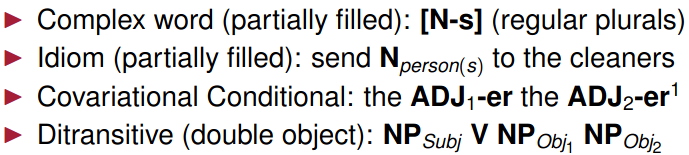
\includegraphics[scale=0.15]{CxG_notation.png}
}\\
\scriptsize{Multiple Constructions} {\tiny
an actual expression typically involves the combination of different constructions\\
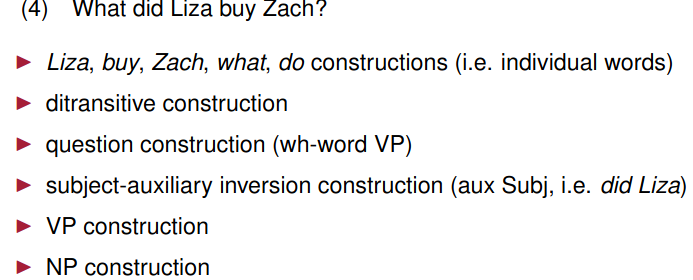
\includegraphics[scale=0.15]{multiple_construc.png}
}\\
\scriptsize{Arguments for Constructions}\\ {\tiny 1. creativity/productivity: the idea that main verbs specify the valency of whole sentences does not match the creative use of linguistic patterns\\
2. non-compositionality: many examples across languages where the overall meaning of a sentence is not derivable from the component parts but is rather assigned to the whole construction\\
3. core and periphery: constructions, while often seen to be part of the periphery, might in fact constitute a core property of language
}\\
\scriptsize{Pros}\\ 
{\tiny not based on an arbitrary distinction between core and periphery of grammar, but tries to cover all linguistic strcutures within the same framework\\
has (arguably) high psycholinguistic relevance for both learning and processing\\
abandons the ideas of headedness and valency, more flexible to deal with the productivity and creativity of languages
}\\
\scriptsize{Cons}\\ 
{\tiny unclear how to identify constructions without recurrence to more traditional analyses such as phrase structure rules and constituency\\
often only partially formalized, Müller argues that all fully formalized CxG variants are virtually equivalent to HPSG(since they largely use the same formal apparatus}